\section{Математическое описание}

\subsection{Конечный автомат}

Управляющий автомат электронных часов зададим набором
\[
    A = (S, \Sigma, Y, s_0, \delta, \lambda),
\]
где $S$ --- множество состояний, $\Sigma$ --- множество входных
воздействий, $Y$ --- множество выходных воздействий, $s_0$ --- начальное
состояние, $\delta: S \times \Sigma \to S$ --- функция переходов,
$\lambda: S \times \Sigma \to Y$ --- функция выходов.

Для варианта 101101132 используются две кнопки $a$ и $b$;
начальное состояние $s_0=S_0$ соответствует отображению текущего времени.
Граф автомата приведён на рисунке~\ref{fig:automaton}. На дугах указаны
входное воздействие и выход автомата в формате «кнопка/микрокоманда».

\begin{figure}[H]
\centering
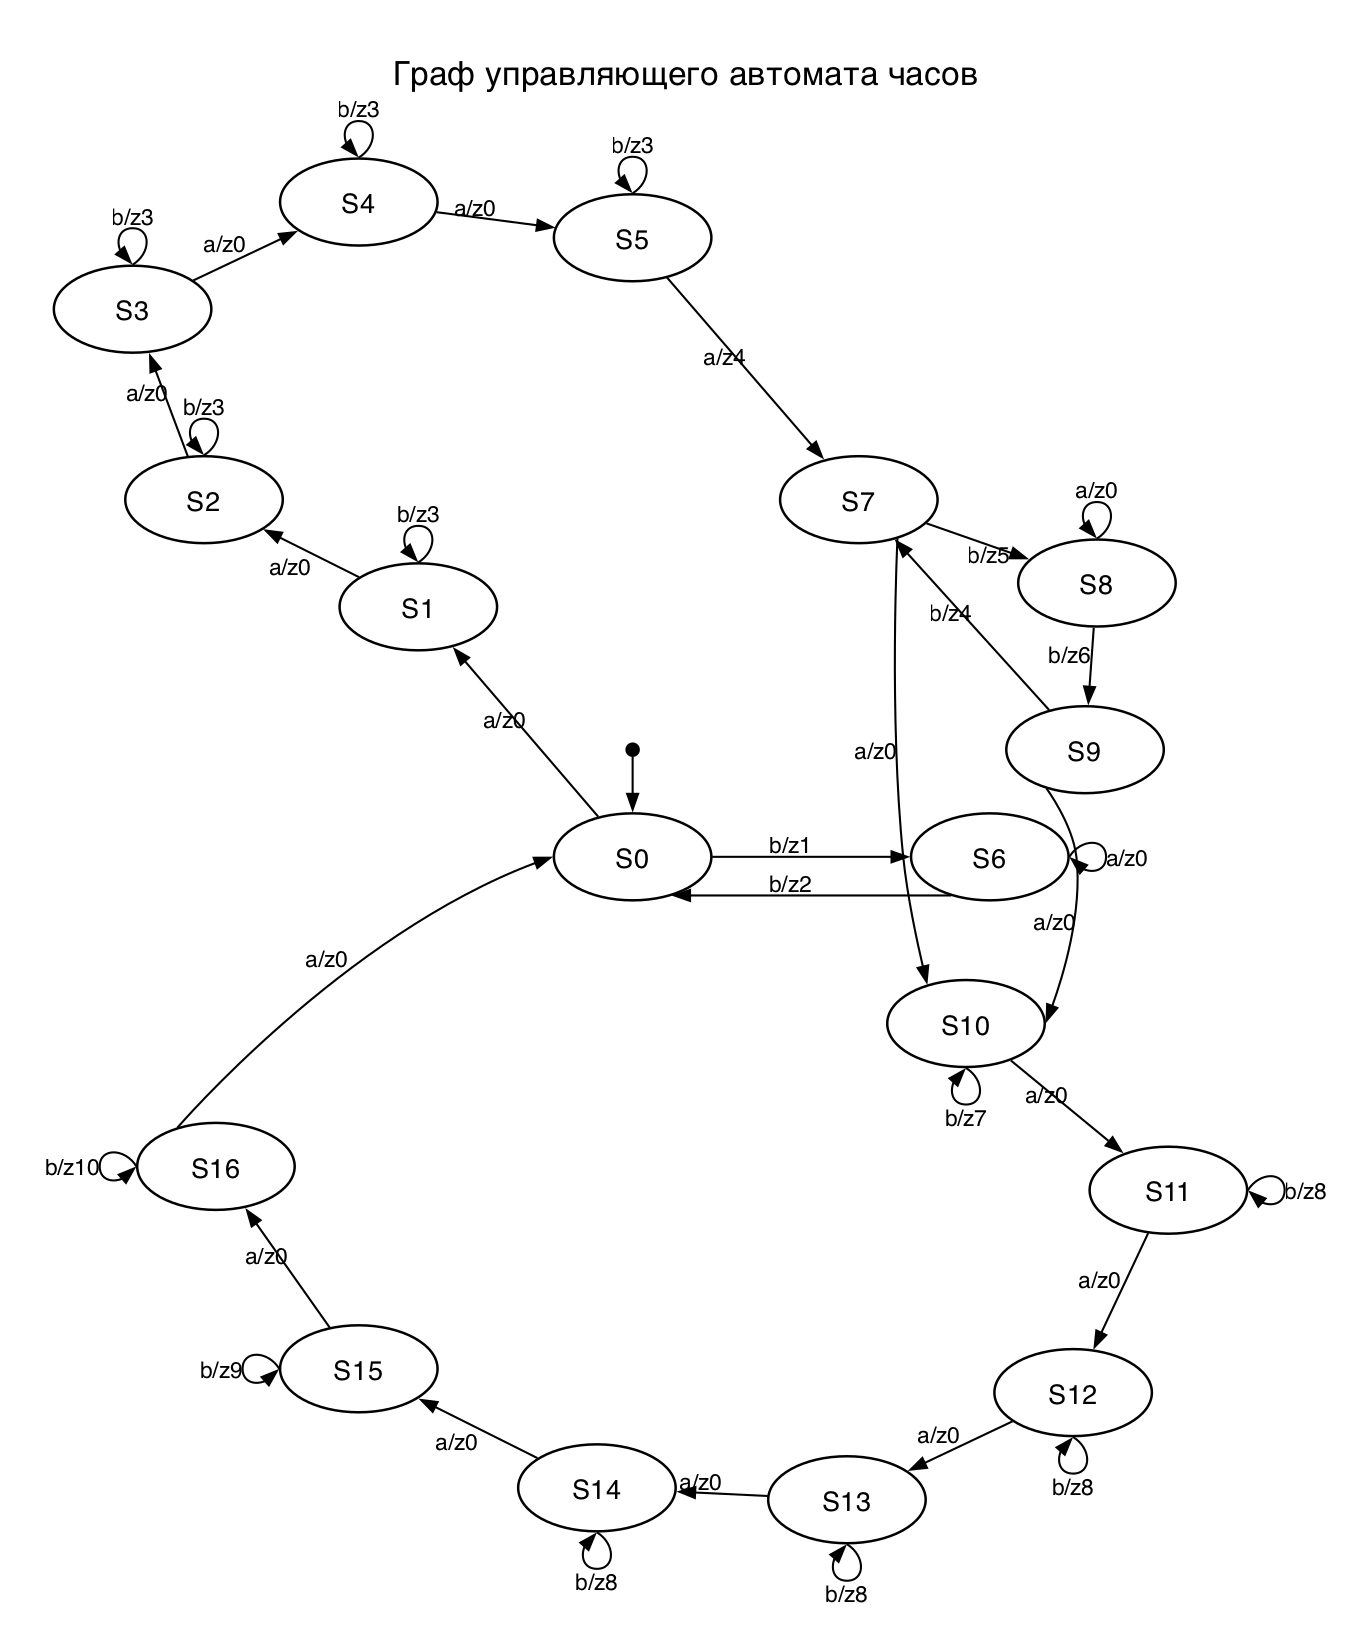
\includegraphics[width=0.7\textwidth]{automaton.png}
\caption{Граф управляющего автомата часов}
\label{fig:automaton}
\end{figure}

Для описываемого автомата:
\begin{itemize}
    \item $S=\{S_0,S_1,S_2,S_3,S_4,S_5,S_6,S_7,S_8,S_9,S_{10},S_{11},S_{12},S_{13},S_{14},S_{15},S_{16}\}$;
    \item $\Sigma=\{a,b\}$;
    \item $Y=\{z_0,z_1,z_2,z_3,z_4,z_5,z_6,z_7,z_8,z_9,z_{10}\}$;
    \item $s_0=S_0$.
\end{itemize}

\subsubsection{Описание состояний автомата}

\begin{enumerate}
    \item $S_0$ --- отображение текущего времени: часов, минут и секунд. При нажатии $a$ автомат переходит в $S_1$ для корректировки десятков часов; при нажатии $b$ часы останавливаются, автомат переходит в $S_6$ и выдаёт $z_1$.
    \item $S_1$ --- корректировка десятков часов. Нажатие $a$ переводит автомат в $S_2$; нажатие $b$ увеличивает выбранный разряд на единицу и выдаёт $z_3$.
    \item $S_2$ --- корректировка единиц часов. Нажатие $a$ переводит автомат в $S_3$; нажатие $b$ увеличивает выбранный разряд на единицу и выдаёт $z_3$.
    \item $S_3$ --- корректировка десятков минут. Нажатие $a$ переводит автомат в $S_4$; нажатие $b$ увеличивает выбранный разряд на единицу и выдаёт $z_3$.
    \item $S_4$ --- корректировка единиц минут. Нажатие $a$ переводит автомат в $S_5$; нажатие $b$ увеличивает выбранный разряд на единицу и выдаёт $z_3$.
    \item $S_5$ --- корректировка секунд. Нажатие $a$ сбрасывает секундомер, автомат переходит в $S_7$ и выдаёт $z_4$; нажатие $b$ увеличивает значение секунд на единицу и выдаёт $z_3$.
    \item $S_6$ --- останов часов. Нажатие $b$ запускает часы, автомат возвращается в $S_0$ и выдаёт $z_2$; нажатие $a$ оставляет автомат в $S_6$ без выходного воздействия $z_0$.
    \item $S_7$ --- секундомер сброшен. Нажатие $b$ запускает секундомер, автомат переходит в $S_8$ и выдаёт $z_5$; нажатие $a$ переводит автомат к настройке будильника в $S_{10}$.
    \item $S_8$ --- секундомер запущен. Нажатие $b$ останавливает секундомер, автомат переходит в $S_9$ и выдаёт $z_6$; нажатие $a$ оставляет секундомер запущенным в $S_8$ без выходного воздействия $z_0$.
    \item $S_9$ --- секундомер остановлен. Нажатие $b$ сбрасывает секундомер, автомат переходит в $S_7$ и выдаёт $z_4$; нажатие $a$ переводит автомат к настройке будильника в $S_{10}$.
    \item $S_{10}$ --- настройка будильника и индикация его состояния. Нажатие $b$ включает или выключает будильник и выдаёт $z_7$; нажатие $a$ переводит автомат в $S_{11}$ для настройки времени будильника.
    \item $S_{11}$ --- корректировка десятков часов будильника. Нажатие $a$ переводит автомат в $S_{12}$; нажатие $b$ увеличивает выбранный разряд на единицу и выдаёт $z_8$.
    \item $S_{12}$ --- корректировка единиц часов будильника. Нажатие $a$ переводит автомат в $S_{13}$; нажатие $b$ увеличивает выбранный разряд на единицу и выдаёт $z_8$.
    \item $S_{13}$ --- корректировка десятков минут будильника. Нажатие $a$ переводит автомат в $S_{14}$; нажатие $b$ увеличивает выбранный разряд на единицу и выдаёт $z_8$.
    \item $S_{14}$ --- корректировка единиц минут будильника. Нажатие $a$ переводит автомат в $S_{15}$; нажатие $b$ увеличивает выбранный разряд на единицу и выдаёт $z_8$.
    \item $S_{15}$ --- выбор мелодии будильника. Нажатие $b$ выбирает следующий номер мелодии и выдаёт $z_9$; нажатие $a$ переводит автомат в $S_{16}$.
    \item $S_{16}$ --- выбор мелодии почасового сигнала. Нажатие $b$ выбирает следующий номер мелодии и выдаёт $z_{10}$; нажатие $a$ возвращает автомат в $S_0$.
\end{enumerate}

Двоичное кодирование состояний приведено в таблице~\ref{tab:states}.

\begin{table}[ht]
\centering
\caption{Состояния управляющего автомата}
\label{tab:states}
\small
\begin{tabular}{|c|p{8cm}|c|}
\hline
Состояние & Назначение & Код $q_1q_2q_3q_4q_5$ \\
\hline
$S_0$  & Отображение текущего времени & 00000 \\
$S_1$  & Корректировка десятков часов & 00001 \\
$S_2$  & Корректировка единиц часов & 00010 \\
$S_3$  & Корректировка десятков минут & 00011 \\
$S_4$  & Корректировка единиц минут & 00100 \\
$S_5$  & Корректировка секунд & 00101 \\
$S_6$  & Останов часов & 00110 \\
$S_7$  & Секундомер сброшен & 00111 \\
$S_8$  & Секундомер запущен & 01000 \\
$S_9$  & Секундомер остановлен & 01001 \\
$S_{10}$ & Настройка и включение/выключение будильника & 01010 \\
$S_{11}$ & Корректировка десятков часов будильника & 01011 \\
$S_{12}$ & Корректировка единиц часов будильника & 01100 \\
$S_{13}$ & Корректировка десятков минут будильника & 01101 \\
$S_{14}$ & Корректировка единиц минут будильника & 01110 \\
$S_{15}$ & Выбор мелодии будильника & 01111 \\
$S_{16}$ & Выбор мелодии почасового сигнала & 10000 \\
\hline
\end{tabular}
\end{table}

Кнопка $a$ переводит автомат к следующему режиму или корректируемому
разряду. Кнопка $b$ изменяет значение либо выполняет действие,
предусмотренное текущим состоянием. Двоичное кодирование входных
воздействий приведено в таблице~\ref{tab:inputs}.

\begin{table}[ht]
\centering
\caption{Входные воздействия автомата}
\label{tab:inputs}
\small
\begin{tabular}{|c|c|}
\hline
Кнопка & Код $x$ \\
\hline
$a$ & 0 \\
$b$ & 1 \\
\hline
\end{tabular}
\end{table}

Множество выходных воздействий $Y=\{z_0,z_1,\ldots,z_{10}\}$. Их назначение
и двоичное кодирование приведены в таблице~\ref{tab:outputs}. Например,
переход $b/z_3$ означает нажатие кнопки $b$ и выдачу импульсной микрокоманды
$z_3$.

\begin{table}[ht]
\centering
\caption{Выходные воздействия управляющего автомата}
\label{tab:outputs}
\small
\begin{tabular}{|c|p{8cm}|c|}
\hline
Выход & Назначение & Код $y_1y_2y_3y_4$ \\
\hline
$z_0$ & Нет импульсного воздействия & 0000 \\
$z_1$ & Останов часов & 0001 \\
$z_2$ & Запуск часов & 0010 \\
$z_3$ & Увеличение выбранного разряда текущего времени на 1 & 0011 \\
$z_4$ & Сброс секундомера & 0100 \\
$z_5$ & Запуск секундомера & 0101 \\
$z_6$ & Останов секундомера & 0110 \\
$z_7$ & Включение или выключение будильника & 0111 \\
$z_8$ & Увеличение выбранного разряда времени будильника на 1 & 1000 \\
$z_9$ & Выбор следующей мелодии будильника & 1001 \\
$z_{10}$ & Выбор следующей мелодии почасового сигнала & 1010 \\
\hline
\end{tabular}
\end{table}

\subsubsection{Функции переходов и выходов}

Функции переходов $\delta: S \times \Sigma \to S$ и выходов
$\lambda: S \times \Sigma \to Y$ автомата приведены в таблице
\ref{tab:transition-output}. Соответствующие переходы показаны на графе
автомата (рисунок~\ref{fig:automaton}).

\begin{table}[H]
\centering
\caption{Функции переходов $\delta$ и выходов $\lambda$}
\label{tab:transition-output}
\small
\setlength{\tabcolsep}{14pt}
\renewcommand{\arraystretch}{1.18}
\begin{tabularx}{\textwidth}{|>{\centering\arraybackslash}X|>{\centering\arraybackslash}X|>{\centering\arraybackslash}X||>{\centering\arraybackslash}X|>{\centering\arraybackslash}X|}
\hline
\rowcolor{tableheaderred}
Состояние & \multicolumn{2}{c||}{\cellcolor{tableheaderred}$\delta$} & \multicolumn{2}{c|}{\cellcolor{tableheaderred}$\lambda$} \\
\cline{2-5}
\rowcolor{tableheaderred}
 & \cellcolor{tableheaderred}$a$ & \cellcolor{tableheaderred}$b$ & \cellcolor{tableheaderred}$a$ & \cellcolor{tableheaderred}$b$ \\
\hline
$S_0$ & $S_1$ & $S_6$ & $z_0$ & $z_1$ \\\hline
$S_1$ & $S_2$ & $S_1$ & $z_0$ & $z_3$ \\\hline
$S_2$ & $S_3$ & $S_2$ & $z_0$ & $z_3$ \\\hline
$S_3$ & $S_4$ & $S_3$ & $z_0$ & $z_3$ \\\hline
$S_4$ & $S_5$ & $S_4$ & $z_0$ & $z_3$ \\\hline
$S_5$ & $S_7$ & $S_5$ & $z_4$ & $z_3$ \\\hline
$S_6$ & $S_6$ & $S_0$ & $z_0$ & $z_2$ \\\hline
$S_7$ & $S_{10}$ & $S_8$ & $z_0$ & $z_5$ \\\hline
$S_8$ & $S_8$ & $S_9$ & $z_0$ & $z_6$ \\\hline
$S_9$ & $S_{10}$ & $S_7$ & $z_0$ & $z_4$ \\\hline
$S_{10}$ & $S_{11}$ & $S_{10}$ & $z_0$ & $z_7$ \\\hline
$S_{11}$ & $S_{12}$ & $S_{11}$ & $z_0$ & $z_8$ \\\hline
$S_{12}$ & $S_{13}$ & $S_{12}$ & $z_0$ & $z_8$ \\\hline
$S_{13}$ & $S_{14}$ & $S_{13}$ & $z_0$ & $z_8$ \\\hline
$S_{14}$ & $S_{15}$ & $S_{14}$ & $z_0$ & $z_8$ \\\hline
$S_{15}$ & $S_{16}$ & $S_{15}$ & $z_0$ & $z_9$ \\\hline
$S_{16}$ & $S_0$ & $S_{16}$ & $z_0$ & $z_{10}$ \\\hline
\hline
\end{tabularx}
\end{table}

В таблице~\ref{tab:binary-transition-output} приведено двоичное
представление переходов и выходов: $x=0$ соответствует кнопке $a$,
$x=1$ --- кнопке $b$; коды состояний и выходов совпадают с кодами,
указанными в таблицах~\ref{tab:states} и~\ref{tab:outputs}.

\begin{table}[H]
\centering
\caption{Двоичное кодирование функций переходов и выходов}
\label{tab:binary-transition-output}
\footnotesize
\setlength{\tabcolsep}{7pt}
\renewcommand{\arraystretch}{1.16}
\begin{tabular}{|c|c|c|c|c|c|c|c|c|c|c|c|c|c|c|c|}
\hline
\rowcolor{tableheaderblue}
\multicolumn{1}{|c|}{\cellcolor{tableheaderblue}\multirow{2}{*}{$S$}} & \multicolumn{1}{c|}{\cellcolor{tableheaderblue}Вход} & \multicolumn{5}{c|}{\cellcolor{tableheaderblue}Текущее состояние} & \multicolumn{5}{c|}{\cellcolor{tableheaderblue}Следующее состояние} & \multicolumn{4}{c|}{\cellcolor{tableheaderblue}Выход} \\
\rowcolor{tableheaderblue}
 & $x$ & $q_1$ & $q_2$ & $q_3$ & $q_4$ & $q_5$ & $Q_1$ & $Q_2$ & $Q_3$ & $Q_4$ & $Q_5$ & $y_1$ & $y_2$ & $y_3$ & $y_4$ \\
\hline
\multirow{2}{*}{$S_0$} & 0 & 0 & 0 & 0 & 0 & 0 & 0 & 0 & 0 & 0 & 1 & 0 & 0 & 0 & 0 \\
\cline{2-16}
 & 1 & 0 & 0 & 0 & 0 & 0 & 0 & 0 & 1 & 1 & 0 & 0 & 0 & 0 & 1 \\
\hline
\multirow{2}{*}{$S_1$} & 0 & 0 & 0 & 0 & 0 & 1 & 0 & 0 & 0 & 1 & 0 & 0 & 0 & 0 & 0 \\
\cline{2-16}
 & 1 & 0 & 0 & 0 & 0 & 1 & 0 & 0 & 0 & 0 & 1 & 0 & 0 & 1 & 1 \\
\hline
\multirow{2}{*}{$S_2$} & 0 & 0 & 0 & 0 & 1 & 0 & 0 & 0 & 0 & 1 & 1 & 0 & 0 & 0 & 0 \\
\cline{2-16}
 & 1 & 0 & 0 & 0 & 1 & 0 & 0 & 0 & 0 & 1 & 0 & 0 & 0 & 1 & 1 \\
\hline
\multirow{2}{*}{$S_3$} & 0 & 0 & 0 & 0 & 1 & 1 & 0 & 0 & 1 & 0 & 0 & 0 & 0 & 0 & 0 \\
\cline{2-16}
 & 1 & 0 & 0 & 0 & 1 & 1 & 0 & 0 & 0 & 1 & 1 & 0 & 0 & 1 & 1 \\
\hline
\multirow{2}{*}{$S_4$} & 0 & 0 & 0 & 1 & 0 & 0 & 0 & 0 & 1 & 0 & 1 & 0 & 0 & 0 & 0 \\
\cline{2-16}
 & 1 & 0 & 0 & 1 & 0 & 0 & 0 & 0 & 1 & 0 & 0 & 0 & 0 & 1 & 1 \\
\hline
\multirow{2}{*}{$S_5$} & 0 & 0 & 0 & 1 & 0 & 1 & 0 & 0 & 1 & 1 & 1 & 0 & 1 & 0 & 0 \\
\cline{2-16}
 & 1 & 0 & 0 & 1 & 0 & 1 & 0 & 0 & 1 & 0 & 1 & 0 & 0 & 1 & 1 \\
\hline
\multirow{2}{*}{$S_6$} & 0 & 0 & 0 & 1 & 1 & 0 & 0 & 0 & 1 & 1 & 0 & 0 & 0 & 0 & 0 \\
\cline{2-16}
 & 1 & 0 & 0 & 1 & 1 & 0 & 0 & 0 & 0 & 0 & 0 & 0 & 0 & 1 & 0 \\
\hline
\multirow{2}{*}{$S_7$} & 0 & 0 & 0 & 1 & 1 & 1 & 0 & 1 & 0 & 1 & 0 & 0 & 0 & 0 & 0 \\
\cline{2-16}
 & 1 & 0 & 0 & 1 & 1 & 1 & 0 & 1 & 0 & 0 & 0 & 0 & 1 & 0 & 1 \\
\hline
\multirow{2}{*}{$S_8$} & 0 & 0 & 1 & 0 & 0 & 0 & 0 & 1 & 0 & 0 & 0 & 0 & 0 & 0 & 0 \\
\cline{2-16}
 & 1 & 0 & 1 & 0 & 0 & 0 & 0 & 1 & 0 & 0 & 1 & 0 & 1 & 1 & 0 \\
\hline
\multirow{2}{*}{$S_9$} & 0 & 0 & 1 & 0 & 0 & 1 & 0 & 1 & 0 & 1 & 0 & 0 & 0 & 0 & 0 \\
\cline{2-16}
 & 1 & 0 & 1 & 0 & 0 & 1 & 0 & 0 & 1 & 1 & 1 & 0 & 1 & 0 & 0 \\
\hline
\multirow{2}{*}{$S_{10}$} & 0 & 0 & 1 & 0 & 1 & 0 & 0 & 1 & 0 & 1 & 1 & 0 & 0 & 0 & 0 \\
\cline{2-16}
 & 1 & 0 & 1 & 0 & 1 & 0 & 0 & 1 & 0 & 1 & 0 & 0 & 1 & 1 & 1 \\
\hline
\multirow{2}{*}{$S_{11}$} & 0 & 0 & 1 & 0 & 1 & 1 & 0 & 1 & 1 & 0 & 0 & 0 & 0 & 0 & 0 \\
\cline{2-16}
 & 1 & 0 & 1 & 0 & 1 & 1 & 0 & 1 & 0 & 1 & 1 & 1 & 0 & 0 & 0 \\
\hline
\multirow{2}{*}{$S_{12}$} & 0 & 0 & 1 & 1 & 0 & 0 & 0 & 1 & 1 & 0 & 1 & 0 & 0 & 0 & 0 \\
\cline{2-16}
 & 1 & 0 & 1 & 1 & 0 & 0 & 0 & 1 & 1 & 0 & 0 & 1 & 0 & 0 & 0 \\
\hline
\multirow{2}{*}{$S_{13}$} & 0 & 0 & 1 & 1 & 0 & 1 & 0 & 1 & 1 & 1 & 0 & 0 & 0 & 0 & 0 \\
\cline{2-16}
 & 1 & 0 & 1 & 1 & 0 & 1 & 0 & 1 & 1 & 0 & 1 & 1 & 0 & 0 & 0 \\
\hline
\multirow{2}{*}{$S_{14}$} & 0 & 0 & 1 & 1 & 1 & 0 & 0 & 1 & 1 & 1 & 1 & 0 & 0 & 0 & 0 \\
\cline{2-16}
 & 1 & 0 & 1 & 1 & 1 & 0 & 0 & 1 & 1 & 1 & 0 & 1 & 0 & 0 & 0 \\
\hline
\multirow{2}{*}{$S_{15}$} & 0 & 0 & 1 & 1 & 1 & 1 & 1 & 0 & 0 & 0 & 0 & 0 & 0 & 0 & 0 \\
\cline{2-16}
 & 1 & 0 & 1 & 1 & 1 & 1 & 0 & 1 & 1 & 1 & 1 & 1 & 0 & 0 & 1 \\
\hline
\multirow{2}{*}{$S_{16}$} & 0 & 1 & 0 & 0 & 0 & 0 & 0 & 0 & 0 & 0 & 0 & 0 & 0 & 0 & 0 \\
\cline{2-16}
 & 1 & 1 & 0 & 0 & 0 & 0 & 1 & 0 & 0 & 0 & 0 & 1 & 0 & 1 & 0 \\
\hline
\end{tabular}
\end{table}

В состояниях корректировки часов, минут и секунд нажатие $b$ увеличивает
соответствующий разряд на единицу. В состоянии $S_0$ нажатие $b$ останавливает
ход часов, а в состоянии $S_6$ --- запускает его. Для секундомера состояния
$S_7$, $S_8$ и $S_9$ задают сброшенное, запущенное и остановленное состояния.
Для выхода из режима секундомера его сначала необходимо остановить.
Сигнал будильника использует выбранную в $S_{15}$ мелодию, почасовой сигнал ---
мелодию, выбранную в $S_{16}$.
